Für eine explizite Berechnung von $\int\limits_M f \mathrm{d}a $
benutzt man idR keine ZdE, sondern zerlegt 
$M = \bigcup\limits_j M_j $ mit $M_j $ paarweise disjunkt und berechnet alle
$\int\limits_{M_j} f \mathrm{d}a $ \\
$\longrightarrow \int\limits_M f \mathrm{d}a 
= \sum\limits_{j=1}^k \int\limits_{M_j} f \mathrm{d}a $

\section{Integralsätze von Gauß und Stokes}

\begin{definition}[Regulärer Randpunkt]
    \mbox{} \\
    Für $\Omega \subset \mathbb{R}^n $ heißt $x \in \partial \Omega $
    \textbf{regulärer Randpunkt} von $\Omega $, falls er eine offene Zylinderumgebung
    $Q \subset \mathbb{R}^n $ besitzt, so dass 
    \emph{nach einer eventuell notwendigen Drehung des Koordinatensystems} gilt:\\
    $Q = Q' \times I $ für $Q' \subset \mathbb{R}^{n-1} $ offen, beschränkt, 
    $I \subset \mathbb{R} $ offenes Intervall und es existiert eine $C^1 $-Funktion
    $h: \tilde{Q}' \rightarrow I $ mit $\tilde{Q}' $ Umgebung von $Q' $
    in $\mathbb{R}^{n-1} $ und \\
    \begin{equation*}
        \Omega \cap Q = 
        \left\lbrace \left(x', x^n \right) \in Q' \times I \ |\ x_n \geq h(x') 
        \right\rbrace
    \end{equation*}        
     
    \begin{equation}
        \partial\Omega \cap Q = 
        \left\lbrace \left(x', x^n \right) \in Q' \times I \ |\ x_n = h(x') \right\rbrace
    \end{equation}
    $x'$ bezeichnet nach Konvention einen (n-1)-dimensionalen Vektor, $x_n$ stellt die
    'fehlende' n-te Komponente dar, $(x', x_n) $ ist also ein n-dimensionaler Vektor.
    Analog wird $Q'$ durch das Intervall $I$ zur Teilmenge vom $\mathbb{R}^n $ ergänzt.
    
    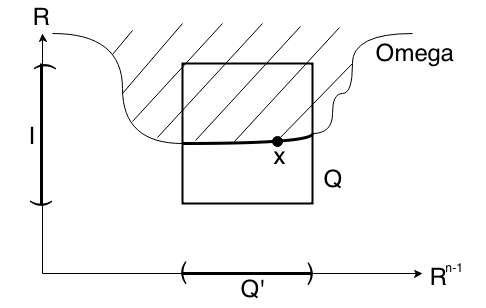
\includegraphics[scale=0.4]{pictures/007-01}
       
    Das heißt in einer Umgebung von $x$ stimmt $\partial \Omega $ mit dem Graphen von $h$
    überein und $\Omega$ liegt über dem Graphen.
    
    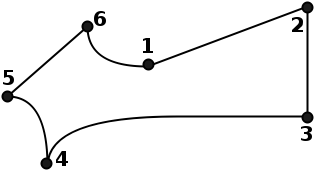
\includegraphics[scale=0.5]{pictures/007-02a}\\
    1: regulärer Randpunkt
    2-6: singuläre Randpunkte\\
    \mbox{}\\
    $\partial_r \Omega $ bezeichnet die \textbf{Menge aller regulären Randpunkte}. \\
    $\partial_s \Omega \coloneqq \partial \Omega / \partial_r \Omega $ ist die 
    \textbf{Menge der singulären Randpunkte}. \\
    $\Gamma \coloneqq \partial \Omega \cap Q \subset \partial_r \Omega $
    gemäß (1) heißt \textbf{glatter} (regulärer) \textbf{Teilrand} von $\Omega$ \\
    falls $\mathcal{L}^{n-1} (\partial \Omega') = 0 $
    für zugehörige $Q' \subset \mathbb{R}^{n-1} $.
\end{definition}    
    
Es ist zu beachten, dass $\partial_r \Omega $ lokal Graph einer
$C^1$-Funktion ist und somit eine (n-1)-dimensionale Mannigfaltigkeit nach Satz 29.1. \\
Für einen glatten Teilrand $\Gamma \subset \partial_r \Omega $ gilt:
$v_{n-1} \left(\overline{\Gamma} / \Gamma \right) = 0 $\\
($\varphi \left(x' \right) = \left(x', h\left(x' \right) \right)
$ ist eine Parametrisierung der Mannigfaltigkeit und \\
$\overline{\Gamma} / \Gamma 
$ ist Bild der (n-1)-dimensionalen Nullmenge $
\partial_r Q' $)

Man erhält eine äquivalente Formulierung zu (1) mittels \\
$\gamma(x) \coloneqq h(x') - x_n \forall (x', x_n) \in Q $ ($Q$, $h$ wie oben) durch
\begin{equation*}
    \Omega \cap Q = \lbrace x \in Q \ |\ \gamma(x) \leq 0 \rbrace
\end{equation*}
\begin{equation}
    \partial \Omega \cap Q = \lbrace x \in Q \ |\ \gamma(x) = 0 \rbrace
\end{equation}

(Dies ist eine lokale Darstellung von $\partial_r \Omega $ als Niveaufläche
und liefert mit Satz 29.4 eine Mannigfaltigkeit, beachte $\gamma'(x) \neq 0 $)

\begin{definition}[Stückweise glatter Rand]
    \mbox{} \\
    $\Omega \subset \mathbb{R}^n $ hat einen \textbf{stückweise glatten Rand}, 
    falls es glatte Teilränder $\Gamma_1, \cdots, \Gamma_m $ von $\Omega$ gibt mit
    $\partial \Omega = \bigcup\limits_{j=1}^m \overline{\Gamma}_j $
\end{definition}

Zum Beispiel haben Würfel oder Polyeder einen stückweise glatten Rand.

Gemäß Bsp. 29.10 erhält man die Einheitsnormalen auf $\partial_r \Omega $
(mit $\gamma$ wie in (2) bzw. $h$ wie in (1)): \\

\begin{equation}
    \nu(x) = 
    \frac{\gamma'(x)}{|\gamma'(x)|} = 
    \frac{(h'(x'),\ -1)}{|(h'(x'),\ -1)|} \
    \forall x \in \partial_r \Omega
\end{equation}

\begin{lemma}
$\forall x \in \partial_r \Omega \exists \delta = \delta(x) > 0$:
\begin{equation}
    x + t \nu(x) \in \mathbb{R}^n / \Omega, \ x - t \nu(x) \in \Omega
    \forall t \in (0, \delta)
\end{equation}
\end{lemma}

\begin{proof}
    Selbststudium.
\end{proof}

Man beachte, dass die Koordinaten in (1), (2) und (3) eventuell bezüglich einem
gedrehten Koordinatensystem zu verstehen sind.

Da in jedem $x \in \partial_r \Omega $ nur zwei Einheitsnormalen existieren, da
$\gamma'(.) $ stetig ist und wegen (4) liefert (3) ein ENF auf der Menge
$\partial_r \Omega $ (insbesondere ist $\nu(.) $ stetig auf $\partial_r \Omega $)

Da alle $\nu(x) $ nach 'außen' zeigen, heißt $\nu$ aus (3) \textbf{äußeres ENF} von
$\partial_r \Omega $.\\
Damit ist $\partial_r \Omega $ mit $\nu$ eine orientierte (n-1)-dimensionale
Mannigfaltigkeit.

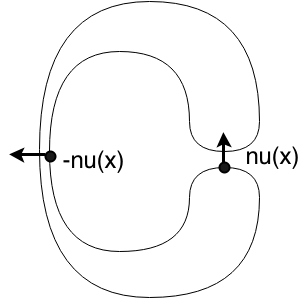
\includegraphics[scale=0.3]{pictures/007-03}

\begin{definition}[Divergenz eines Vektorfelds]
    \mbox{} \\
    Eine Abbildung $F: \mathbb{R}^n \rightarrow \mathbb{R}^n $ heißt auch
    \textbf{Vektorfeld}.\\
    Falls $F$ in $x \in M $ differenzierbar ist, heißt \\
    $\mathrm{div\ }F(x) \coloneqq \pdiff{F_1}{x_1}(x) + \cdots + \pdiff{F_n}{x_n}(x) =
    \mathrm{tr\ }\left(F'(x)\right) $\\
    \textbf{Divergenz} des Vektorfelds $F$ in $x$.
\end{definition}

\begin{satz}[Gaußscher Integralsatz - Spezialfall für Quader]
\mbox{} \\
Sei $F: U \subset \mathbb{R}^n \rightarrow \mathbb{R}^n $ ein stetig differenzierbares VF,
$U$ sei offen, $Q \subset \mathbb{R}^n $ ein Quader, $\overline{Q} \subset U \\
$
\begin{equation}
    \Longrightarrow 
    \underbrace
        {\int\limits_Q \mathrm{div\ } F(x) \mathrm{d}x
    }_{
        \text{Lebesgue-Integral in }\mathbb{R}^n}
    =
    \underbrace{
        \int\limits_{\partial Q} F(x) \nu(x) \mathrm{d}a
    }_{
        \text{Integral auf (n-1)-dim. Fläche } \partial Q
    }    
\end{equation}

\end{satz}

Gelegentlich schreibt man auch $\int\limits_{\partial Q} F \ \mathrm{d}\vec{a} $ anstatt
der rechten Seite in (5) und bezeichnet
$\mathrm{d}\vec{a} = \nu \mathrm{d}a $ als vektorielles Flächenelement auf
$\partial Q $.

\textbf{Interpretation bei n = 1:}\\
$Q = (a,b) \subset \mathbb{R}, \ \mathrm{div\ } F(x) = F'(x) $ \\
Man kann $\partial Q = \lbrace a, b \rbrace $ 
als 0-dimensionale Mannigfaltigkeit betrachten,\\
$\nu(b) = 1, \ \nu(a) = -1 $\\
in (5) wäre dann
$\int\limits_a^b F'(x) \mathrm{d}x = F(b) - F(a) $\\
Das heißt der Hauptsatz der Differential- und Integralrechnung ist
ein Spezialfall des Gaußschen Integralsatzes!

\begin{proof}
\mbox{} \\
Sei $\nu(x) = (\nu_1(x), \cdots, \nu_n(x)) $\\
Wir zeigen für beliebige $C^1$-Funktionen $f: U \rightarrow \mathbb{R} $,
dass gilt: \\
\begin{equation}
    \int\limits_Q \pdiff{}{x_k} f(x) \mathrm{d}x =
    \int\limits_{\partial Q} f(x) \nu_k (x) \mathrm{d}a
\end{equation}
Ersetzt man hier $f$ durch $F_k$ und summiert über über $k$ so folgt (5).\\
Zeige (6) (oBdA sei $k=n$):
Sei $Q = Q' \times (a,b), \ Q' \subset \mathbb{R}^{n-1} $ Quader\\
Auf $\partial_r Q $ hat man
$\nu_n (x) = 
\begin{cases}
    1 \text{ auf } Q' \times \lbrace b \rbrace \\
    -1 \text{ auf } Q' \times \lbrace a \rbrace \\
    0 \text{ auf } \partial Q' \times (a,b)
\end{cases}
$
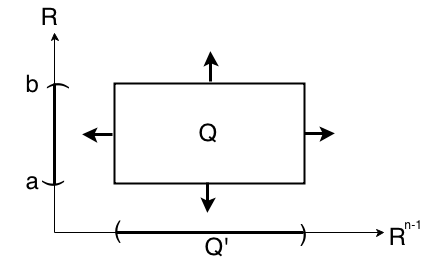
\includegraphics[scale=0.3]{pictures/007-04}

$\Rightarrow \int\limits_{\partial Q} \nu_n f \mathrm{d}a =
\int\limits_{Q' \times \lbrace b \rbrace} f \mathrm{d}a -
\int\limits_{Q' \times \lbrace a \rbrace} f \mathrm{d}a
$ \\
Nun parametrisiert man die Mannigfaltigkeiten 
$Q' \times \lbrace a \rbrace $ bzw. $ Q' \times \lbrace b \rbrace $ durch \\
$x' \rightarrow (x', a) $ bzw. $x' \rightarrow (x', b) $ mit $x' \in Q' $ \\
Offenbar ist die Gramsche Determinante jeweils 1. \\
$\Rightarrow 
\int\limits_{\partial Q} f \nu_n \mathrm{d}a =
\int\limits_{Q'} f(x',b) \mathrm{d}x' -
\int\limits_{Q'} f(x',a) \mathrm{d}x' \\
\stackrel{\text{HS Int'rechnung}}{=}
\int\limits_{Q'} \left(
\int\limits_a^b \pdiff{}{x_n} f(x', \psi) \mathrm{d}\psi \right) \mathrm{d}x' \\
\stackrel{\text{Fubini}}{=} \int\limits_Q \pdiff{}{x_n} f(x) \mathrm{d}x
\Rightarrow $ (6) $\Rightarrow $ Behauptung.
\end{proof}